% 進捗報告用の全体まとめ（修論 Method / Results and Discussion の日本語版）
% 文体・用語・表は progress_report_2026-08-09_topic.tex（加藤先生確認済み）を踏襲。
% 数値はすべて experiments/*.json と照合済み（各節の出典は修論の % source: コメントに対応）。
% LLM 直接生成の帰属は 2026-08-31 訂正後（生成 claude-sonnet-4-5・判定 claude-opus-4-8 別モデル）。
\documentclass[11pt,a4paper]{ltjsarticle}
\usepackage{luatexja-fontspec}
\usepackage{geometry}
\usepackage{booktabs}
\usepackage{array}
\usepackage{enumitem}
\usepackage{graphicx}
\usepackage{amsmath}
\usepackage{fancyhdr}
\usepackage{xcolor}
\usepackage{hyperref}

\geometry{margin=24mm}
\setmainjfont[BoldFont=Hiragino Kaku Gothic ProN]{Hiragino Mincho ProN}
\setsansjfont{Hiragino Kaku Gothic ProN}
\setmonofont{Menlo}
\hypersetup{colorlinks=true, linkcolor=blue!55!black, urlcolor=blue!55!black}

\pagestyle{fancy}
\fancyhf{}
\lhead{研究進捗報告}
\rhead{2026 年 8 月 31 日}
\cfoot{\thepage}
\renewcommand{\headrulewidth}{0.2pt}

\newcommand{\rk}{\textrm{Recall@}K}
\setlist{nosep}

\begin{document}

\begin{center}
{\sffamily\large 物理モデルの自動構築：手法と結果・考察の全体まとめ}
\end{center}
\vspace{0.3em}
\hfill 作成者：M2\ 一洋
\vspace{0.8em}

%======================================================================
\section{本報告の位置づけ}
%======================================================================
\textbf{研究の目的}：科学文献から数式を集めておき、「どんな物理モデルを作りたいか」（説明文と入出力変数）を入力すると、そのモデルを構成するのに必要な\textbf{数式の集合}を提示する。

本報告は、手法（\S\ref{sec:method}）・データと評価方法（\S\ref{sec:data}）・現時点までの結果と考察（\S\ref{sec:overall}〜\S\ref{sec:limits}）を 1 つにまとめた全体版である。\S\ref{sec:greedy}〜\S\ref{sec:error} はこれまでのゼミ報告に載せていなかった結果、\S\ref{sec:redesign} は今回新たに行なった実験である。

%======================================================================
\section{手法}\label{sec:method}
%======================================================================
\subsection{課題の定式化}
入力は、作りたいモデルの説明文と、与えられる変数（入力変数）・求めたい変数（出力変数）である。データベースの $11{,}146$ 式の中から、そのモデルを構成する正解の式集合（$K$ 本）を選び出す。物理モデルは独立な式の寄せ集めではなく、変数を共有し連立して解く\textbf{系}なので、選んだ式集合が「解ける形」かどうかも問う。本報告では、出力変数がすべて式に現れ、かつ\textbf{未知の変数の数が式の数以下}（入力変数を与えれば残りが一意に決まる状態）のとき、その式集合は\textbf{閉じている}（自由度ゼロ）と言う。

\subsection{第 1 段：候補の絞り込み}\label{sec:stage1}
第 1 段では、データベースの全式に、説明文と式まわりの文章がどれだけ似ているか（\textbf{文章類似度}）と、指定された入出力変数と式の変数がどれだけ重なるか（\textbf{変数の一致度}）に、それぞれ $0.7$ と $0.3$ の重みを掛けて足した点数を付け、上位 $k=50$ 件を候補として絞り込む。

正解式のうち候補 50 件に入った割合を\textbf{被覆率}と呼ぶ。第 2 段は候補の中しか並べ直せないので、\textbf{被覆率は第 2 段の精度の上限}を与える。現行の重みでの被覆率は $0.920$ である（1{,}823 ケースの平均。この上限は \S\ref{sec:redesign} の主題になる）。

\subsection{第 2 段：10 個の特徴量による並べ直し}
第 2 段では、候補 50 件だけを対象に、10 個の特徴量を多層パーセプトロン（MLP、隠れ層 64 ユニット 2 層）で点数化して並べ直す。学習は「正解式の点数を、同じ候補内の不正解式より上げる」ペア比較の損失で行なう。10 個の特徴量の意味と計算方法を表~\ref{tab:features} にまとめる。

\begin{table}[h]\centering
\footnotesize
\caption{第 2 段が使う 10 個の特徴量。式が持つ変数の集合を $V_e$、入力で指定された入出力変数の集合を $V_q$（入力 $V_{\mathrm{in}}$・出力 $V_{\mathrm{out}}$）、参照集合の式が持つ変数の集合を $V_S$ とする。}
\label{tab:features}
\begin{tabular}{@{}lp{0.63\linewidth}@{}}
\toprule
特徴量 & 意味と計算方法 \\
\midrule
\multicolumn{2}{@{}l}{\textbf{基本の 7 個}：候補の式を 1 本ずつ、入力と照らして評価する}\\
文章類似度 & 説明文と式まわりの文章の、TF-IDF で重み付けした単語ベクトルのコサイン類似度 \\
意味の近さ & 同じ 2 つの文章を 256 次元に圧縮（TF-IDF ＋ SVD）したベクトルのコサイン類似度。単語が一致しなくても内容が近ければ大きい \\
分野の一致 & 式に付いた分野名が説明文に現れれば $1$、なければ $0$ \\
変数の一致度 & 入出力変数と式の変数がどれだけ重なるか。$|V_q\cap V_e|/|V_q\cup V_e|$（Jaccard 係数） \\
入力変数の被覆 & 入力変数のうち式に現れる割合。$|V_{\mathrm{in}}\cap V_e|/|V_{\mathrm{in}}|$ \\
出力変数の被覆 & 出力変数のうち式に現れる割合。$|V_{\mathrm{out}}\cap V_e|/|V_{\mathrm{out}}|$ \\
式の特化度 & 式の変数のうち入出力変数が占める割合。$|V_q\cap V_e|/|V_e|$。無関係な変数を持たない式ほど大きい \\
\addlinespace
\multicolumn{2}{@{}l}{\textbf{集合の 3 個}：第 1 段で上位 5 件に入った式を参照集合とし、それとの関係で評価する}\\
補完性 & 参照集合がまだ覆っていない入出力変数を、その式が新たに補う割合。$|(V_q\cap V_e)\setminus V_S|/|V_q|$ \\
一貫性 & 式の変数のうち参照集合と共有する割合。$|V_e\cap V_S|/|V_e|$ \\
分野の一致（集合版） & 参照集合の式のうち、その式と分野名が同じものの割合 \\
\bottomrule
\end{tabular}
\end{table}

\subsection{逐次選択}\label{sec:seqmethod}
集合の 3 特徴量は「参照集合との関係」で決まるが、上の並べ直しでは参照集合を第 1 段の上位 5 件に\textbf{固定}している。これに対し\textbf{逐次選択}では、式を 1 本選ぶごとに、集合の 3 特徴量を「既に選んだ式」を参照集合にして計算し直し、次の 1 本を選ぶ。さらに\textbf{学習も逐次の手順}で行なえる：学習時に正解の式を 1 本ずつ既選択に加えながら、各段階で「次の正解式」を不正解式より上に押し上げるよう学習する。これにより、学習と推論が同じ問い（「これらを選んだ今、系を閉じるために次に要る式はどれか」）を解くようになる。

\subsection{自由度ゼロ停止}
並べ直しは「何本返すか」を利用者が知っている前提に立つが、モデル構築では式の本数こそ知りたい量である。そこで、逐次選択で 1 本選ぶごとに「選んだ集合が閉じたか」（出力変数をすべて含み、未知の変数の数 $\le$ 式の数）を確かめ、\textbf{閉じた時点で自動的に止まる}規則を加えた。返す集合は構成上「解ける形」で閉じている。

%======================================================================
\section{データセットと評価方法}\label{sec:data}
%======================================================================
\subsection{数式データベースと評価ケース}
データベースは 361 文献（論文 PDF 328 件＋分野別の基礎式集 33 件）から抽出した $11{,}146$ 式である。抽出は LLM（Gemini 2.5 Pro）が行ない、各式は「式・変数の集合・式まわりの文章・出典・分野名」を持つ。変数は記号の完全一致で照合し、表記の正規化は行なっていない（$C_A$ と $C_A(t)$ は別変数として扱う）。

評価ケースは表~\ref{tab:cases} の 3 種類、計 1{,}823 件である。呼び方は正解集合の作り方に沿ってそろえた（これまでの報告の「オリジナル」を\textbf{文献掲載}、「DAE」を\textbf{合成}と呼ぶ。中身は同じ）。このほか、既存ケースの入出力の入替や説明文の言い換えで作った拡張ケース 1{,}015 件を\textbf{訓練にのみ}使う。拡張を評価に入れると易しい複製で点が水増しされるため（差が $+0.222$ から $+0.156$ に縮んで見える）、評価からは除外した。

\begin{table}[h]\centering
\small
\caption{評価ケースの 3 種類。「式数」は正解集合の平均本数（括弧は最大）。}
\label{tab:cases}
\begin{tabular}{@{}llcc@{}}
\toprule
種類 & 正解集合の作り方 & 件数 & 式数 \\
\midrule
文献掲載 & 文献が 1 つのモデルとして掲載している式集合をそのまま使う & 92 & 1.34 (4) \\
文献横断 & 異なる文献の式を、共有する変数でつないで作る & 731 & 2.03 (3) \\
合成 & 微分方程式から出発し、変数を共有する式を足して指定サイズ $X$ の & 1{,}000 & 5.50 (10) \\
     & \quad 閉じた系に育てる（$X=1$〜$10$ 各 100 件。解けることが構成上保証） & & \\
\bottomrule
\end{tabular}
\end{table}

評価は\textbf{設定 A}（3 種類すべて、1{,}823 件）と\textbf{設定 B}（合成のみ、1{,}000 件＝正解集合が最も大きく最難）で行なう。1{,}823 件のうち 90.8\% は正解が 2 式以上で、平均は 3.90 式である。

\subsection{分割・指標・比較手法}
訓練とテストは\textbf{文献単位}で分ける（同じ文献のケースが両側に入ると答え漏れになるため）。分け方は 400 通りの無作為候補から、難しさに関わる 4 つの分布（正解式数・入力変数数・出力変数数・出典数）が訓練とテストで最もそろう 1 通りを選ぶ（層化）。すべての実験を同じ乱数 10 通りで繰り返し、平均と乱数間のばらつきを報告する。差の検定には乱数 10 通りの対応を取った Wilcoxon 符号順位検定を使う（$n=10$ の最小 $p$ 値は $0.00195$ で、これは「10 通りすべてで勝った」ことを意味する）。

主指標は $\rk$（正解式数 $K$ に合わせ、上位 $K$ 件に入った正解式の割合。情報検索でいう R-precision）である。補助として MAP（Mean Average Precision）と Recall@20 も報告する。自由度ゼロ停止は「集合」を返すので、完全一致率（返した集合が正解集合と完全に一致した割合）・集合 F1・閉包率（返した集合が閉じている割合）で評価する。

比較手法は次の 3 つである。\textbf{古典的情報検索手法（baseline）}は、第 1 段と同じ点数（文章類似度 $0.7$＋変数の一致度 $0.3$）で全 $11{,}146$ 式を並べる（学習なし・候補の絞り込みなし）。\textbf{LLM 直接生成}は、同じ入力を LLM（claude-sonnet-4-5）に与えて必要な式をそのまま書かせる。生成された式が正解式と数学的に等価かは\textbf{別の上位モデル}（claude-opus-4-8）が判定し、等価なら正解と数えて同じ指標で採点する（判定に費用がかかるため各設定約 50 件の一様サンプル）。\textbf{本手法（reranker-10S）}は \S\ref{sec:method} の 2 段構えである。

%======================================================================
\section{結果 1：全体比較 --- 難しいケースほど差が開く}\label{sec:overall}
%======================================================================
表~\ref{tab:overall} に全体比較を示す。本手法は $\rk$ を設定 A で $0.521 \to 0.743$（$+0.222$）、設定 B で $0.466 \to 0.689$（$+0.223$）に上げ、どちらも乱数 10 通りすべてで baseline を上回った（Wilcoxon $p=0.00195$）。LLM 直接生成は $0.254$（A）・$0.226$（B）にとどまる。ただし順位を問わず「等価な式をどこかに書けたか」で数えると 0.419（A）・0.343（B）に達するので、LLM は\textbf{式を書けないのではなく、正解 $K$ 本の集合として組めない}。また正解式には特定の文献で係数を当てはめた経験式が多く、その文献を読んでいない生成器は同じ式を書けない。検索はこの点で有利である。

\begin{table}[h]\centering
\small
\caption{全体比較（$\rk$ は乱数 10 通りの平均$\pm$標準偏差）。LLM 直接生成は各設定約 50 件の一様サンプルによる 1 回評価のため、ばらつきと MAP・Recall@20 は付さない。}
\label{tab:overall}
\begin{tabular}{@{}llccc@{}}
\toprule
設定 & 手法 & $\rk$ & MAP & Recall@20 \\
\midrule
A（1{,}823 件） & 古典的情報検索手法（baseline） & $0.521 \pm 0.045$ & 0.581 & 0.836 \\
 & LLM 直接生成（$n=48$） & 0.254 & --- & --- \\
 & \textbf{本手法（reranker-10S）} & $\mathbf{0.743 \pm 0.054}$ & \textbf{0.863} & \textbf{0.909} \\
\midrule
B（合成のみ 1{,}000 件） & 古典的情報検索手法（baseline） & $0.466 \pm 0.037$ & 0.512 & 0.721 \\
 & LLM 直接生成（$n=50$） & 0.226 & --- & --- \\
 & \textbf{本手法（reranker-10S）} & $\mathbf{0.689 \pm 0.033}$ & \textbf{0.832} & \textbf{0.838} \\
\bottomrule
\end{tabular}
\end{table}

差はケースが難しいほど開く。正解が 1 式のケースでは baseline $0.849$ 対 本手法 $0.878$（差 $+0.03$）でほぼ並ぶが、正解式数が増えると baseline は 10 式で $0.281$ まで落ち、本手法は $0.543$ にとどまる（差 $+0.21$〜$+0.29$）。入力変数数でも差は $+0.05$（5 個以下）から $+0.28$（21 個以上）へ広がる。つまり\textbf{1 本の式を探す課題はほぼ解けており、本手法の価値は「集合として選ぶ」難しいケースにある}。

%======================================================================
\section{結果 2：向上の内訳と、モデルが実際に頼っている特徴量}\label{sec:mech}
%======================================================================
設定 A の $+0.222$ は 3 段に分解できる。\textbf{(i) 重みの学習}：baseline と同じ 2 特徴量（文章類似度・変数の一致度）だけを MLP で学習し直すと $0.521 \to 0.601$（$+0.080$）。\textbf{(ii) 特徴量の追加}：基本 7 個にすると $0.601 \to 0.693$（$+0.092$）。ただし\textbf{式の特化度を 1 つ足すだけで $0.691$（$+0.090$）}に達し、この段はほぼ特化度 1 本が担う。\textbf{(iii) 集合の特徴量}：3 個を足すと $0.693 \to 0.743$（$+0.050$、Wilcoxon $p=0.00195$）。内訳は補完性 $+0.052$・一貫性 $+0.050$（各 $p=0.00195$）で、この 2 つは互いに代わりが利く（3 つ足しても 1 つ分しか上がらない）。\textbf{分野の一致（集合版）は $-0.000$（$p=0.98$）で寄与しない}。

集合特徴量の上乗せ $+0.050$ は一様ではない。正解が 1 式のケースではゼロ（参照集合が役立ちようがない）、正解 3 式で最大（$+0.102$）、そして\textbf{最難端（入力 16 変数以上）では $+0.035$ に半減}する（11--15 変数では $+0.078$）。この頭打ちへの対処は \S\ref{sec:greedy} で述べる。

各特徴量の重要度は、\textbf{訓練済みモデルの入力のうち 1 つの特徴量の値だけを候補間で無作為に入れ替え（シャッフル）、$\rk$ の低下を測る}方法（PFI、Permutation Feature Importance）でも確かめた（図~\ref{fig:pfi}）。変数の重なりを測る 6 特徴量をまとめてシャッフルすると $\rk$ は $0.743 \to 0.065$ に崩れる（低下 $+0.678$、$p<0.001$）。話題の近さを測る 4 特徴量ではまとめても $+0.006$（$p=0.10$、有意でない）。\textbf{特徴量を足して訓練し直す方法（アブレーション）と、訓練済みモデルを壊す方法（PFI）が同じ結論に至った}：効くのは変数の重なりであり、話題の近さではない。

\begin{figure}[h]\centering
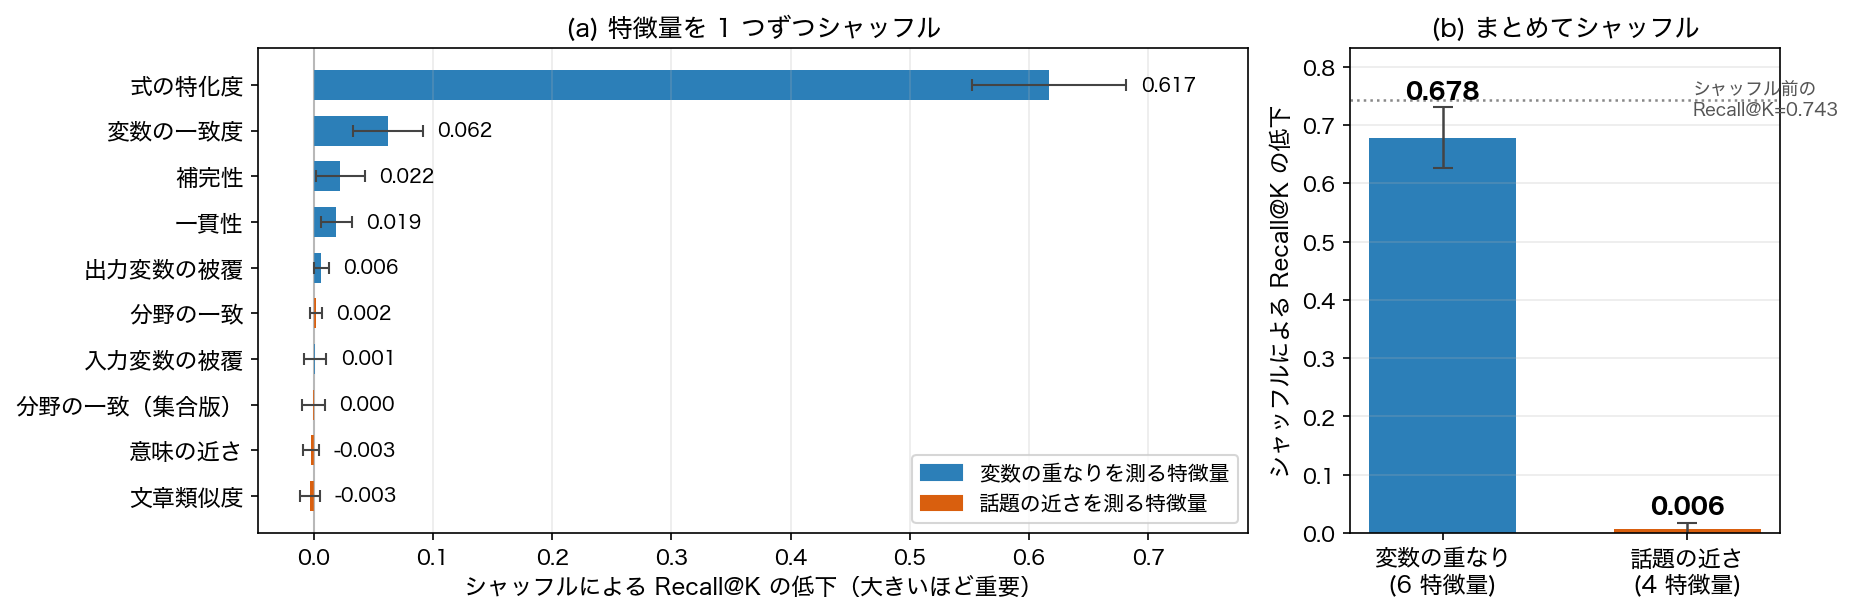
\includegraphics[width=0.80\linewidth]{figures/fig_pfi_importance.png}
\caption{特徴量の値をケース内でシャッフルしたときの $\rk$ の低下（大きいほどモデルがその特徴量に頼っている）。誤差棒は乱数 10 通りの標準偏差。(b) の点線はシャッフル前の $\rk = 0.743$。}
\label{fig:pfi}
\end{figure}

%======================================================================
\section{結果 3：逐次選択は最難ケースの頭打ちを解く}\label{sec:greedy}
%======================================================================
\S\ref{sec:mech} の頭打ちの原因を「参照集合を第 1 段の上位 5 件に固定しているため、長い正解集合では参照が実際の選択と食い違っていくから」と推定し、\S\ref{sec:seqmethod} の逐次選択で介入した。この比較は候補を $k=200$ 件に広げて行なう（被覆率の上限が $0.920 \to 0.978$ に上がるため、数値は表~\ref{tab:overall} の $k=50$ とは直接比べない）。

設定 B（合成のみ）で、参照固定 $0.724 <$ 選び方のみ逐次 $0.756 <$ \textbf{学習も逐次 $0.765$} となった（10 乱数）。学習を逐次にする上乗せ $+0.009$ は有意である（Wilcoxon $p=0.037$）。そして\textbf{効き目は予測した場所に集中する}：正解 8 式以上のケースで、学習版逐次は参照固定を $+0.056$ 上回る（$p=0.00195$）。設定 A でも $0.757 < 0.787 < 0.797$ と同じ並びになる（ただし A では学習版と選び方のみの差 $+0.010$ に有意差は認められない、$p=0.13$）。「頭打ちの原因を推定し、そこだけ直す介入をし、予測した場所で回復する」という手順で、集合特徴量が効いている仕組みを確かめた。

%======================================================================
\section{結果 4：式の本数を教えなくても、解ける集合を返して自分で止まる}\label{sec:dof}
%======================================================================
自由度ゼロ停止（$K$ を教えない）を、同じ学習版逐次モデルで「$K$ を教えて上位 $K$ 本を返す場合」と比べた。\textbf{完全一致率は $K$ を教えた場合と完全に同じ}（設定 A $0.526$、設定 B $0.368$。全ケース・全乱数の延べ 7{,}026 件で判定が 1 件も食い違わない）。理由は単純で、完全に正しい選択は閉じた系そのものだから、閉じた時点で止まれば同じ集合になる。集合 F1 の低下はわずかで（A $-0.008$、B $-0.023$、対応 $t$ 検定 $p=0.006$・$0.0001$）、一方\textbf{閉包率は $K$ を教えた場合より高い}（A $0.936$ 対 $0.865$、B $0.883$ 対 $0.781$）：上位 $K$ 本は解ける保証がないが、自由度ゼロ停止は閉じるまで選び続けるからである。止まる位置の誤りは中央値 0 で、誤るときはほぼ全て多めに選ぶ方向であった（設定 B は誤った 545 件すべて、設定 A は 4{,}594 件中 1 件だけ少なめ）。

正直な注記：本データでは正解式数が出力変数数とほぼ等しい（文献横断・合成で 100\%）ため、「$K$ を当てること」自体は難しくない。主張は $K$ 予測ではなく、\textbf{自分で止まれること}と\textbf{返す集合が解ける形で閉じている保証}である。

%======================================================================
\section{結果 5：話題の近さはなぜ効かないか（原因のまとめと新しい発見）}\label{sec:topic}
%======================================================================
話題を見る 4 特徴量（文章類似度・意味の近さ・分野の一致・同集合版）は、どの形でも第 2 段に寄与しない：分野の一致を 2 特徴量に足しても $+0.002$（$p=0.06$）、意味の近さでは $-0.002$（$p=0.48$）、集合版は $-0.000$（$p=0.98$）。分野名を統合して粗くしても（1{,}958 群・100 群・40 群）寄与は最大 $+0.0006$ で全て $p>0.6$ である。原因は前回までに報告した 2 つに加え、今回 1 つを追加できた。

\textbf{(1) 絞り込みの後では話題がそろってしまう（既報）}：意味の近さ 1 つで正解式を並べる力（AUC、正解式が不正解式より高い値を取る組の割合）は、全データベース相手なら $0.950$ あるのに、候補 50 件の中では $0.594$ に落ちる（表~\ref{tab:auc}）。話題の仕事は第 1 段の絞り込みで終わっている。\textbf{(2) 選抜が作る見かけの逆相関（既報）}：候補は「文章類似度＋変数の一致度が高い式」だけの集合なので、その中では文章類似度の高さが変数の合わなさの裏返しになり（相関 $-0.404$）、文章類似度は候補内でわずかに逆向きの信号になる（AUC $0.437$）。

\begin{table}[h]\centering
\small
\caption{1 つの特徴量だけで正解式を不正解式より上に並べられる割合（AUC、1{,}823 ケースの平均$\pm$標準誤差）。列は不正解式の範囲の違いを表す。}
\label{tab:auc}
\begin{tabular}{lcc}
\toprule
特徴量 & 全データベース $11{,}146$ 式 & 候補 50 件の中 \\
\midrule
変数の一致度 & $0.999 \pm 0.000$ & $0.947 \pm 0.002$ \\
式の特化度 & — & $0.965 \pm 0.001$ \\
意味の近さ & $0.950 \pm 0.003$ & $0.594 \pm 0.006$ \\
文章類似度 & $0.913 \pm 0.003$ & $0.437 \pm 0.007$ \\
\bottomrule
\end{tabular}
\end{table}

\textbf{(3) 全体ゼロの正体は「打ち消し合い」だった（今回報告）}：分野の一致（集合版）の重要度をケースごとに分けて見ると、候補の中でこの特徴量の値が正解式側で高いケース（1{,}169 件）ではシャッフルで $\rk$ が $0.012$ \textbf{下がり}、不正解式側で高いケース（414 件）では逆に $0.034$ \textbf{上がる}（Mann--Whitney の $U$ 検定、$p=1.3\times10^{-8}$。同じケースが複数の乱数に現れる分は 1 件に集約して数えた）。加重平均するとちょうどゼロになる。つまりモデルはこの特徴量を\textbf{ケースごとには使っており、役立つケースと精度を下げるケースが打ち消し合って}全体でゼロに見える。分野名の統合で消えなかったのだから、この特徴量を生かすには「正しい向きを向くケース」を増やす別の工夫が要る。

%======================================================================
\section{結果 6：残る誤りはどこで生まれるか}\label{sec:error}
%======================================================================
取り逃した正解式がどこで漏れたかを 1 分割（乱数 42、テスト 423 件、取り逃し 435 本）で数えると、\textbf{61.8\% は第 1 段で候補 50 件に入らず}、38.2\% が候補に入ったのに上位 $K$ 件から漏れた。候補を 200 件に広げると比率は逆転し（第 1 段 28.4\%・並べ直し 71.6\%）、取り逃し自体は 373 本に減る。つまり $k=50$ の主要比較では第 1 段が、$k=200$ の逐次選択では並べ直しが、それぞれ誤りの主因である。

解けないケースは種類ではなく大きさで決まる：解けたケースの正解は平均 2.13 式・入力 10.8 変数、落ちたケースは 5.34 式・17.8 変数で（どちらも Mann--Whitney $p<10^{-14}$）、落ちたケースは被覆率自体が $0.83$ に下がっている（解けたケースは $1.00$）。並べ直しで漏れた正解式は、いま持っているどの特徴量でも救えない：漏れた正解式とその上に居た不正解式の組で、正解側の値が高い割合は意味の近さで $0.516$（偶然と同水準）、変数の一致度では $0.375$（むしろ不正解側が高い）である。

残る誤りには 2 つの型がある。\textbf{型 1：別文献の同一式}。標準的な式は文献をまたいで繰り返し現れるため、数学的に同一の式を別文献から選んでしまう（例：回分発酵の $\mathrm{d}X/\mathrm{d}t=\mu X$ で、別文献に載った同じ増殖式が上位に来た。話題の近さはむしろ誤り側を推す）。\textbf{型 2：式の向き}。特徴量は変数の集合しか見ないため、同じ変数から\textbf{別の変数を決める}2 本の式（例：線形化した反応器の $\mathrm{d}C_A'/\mathrm{d}t$ の式と $\mathrm{d}T'/\mathrm{d}t$ の式）が全特徴量で同点になる。どちらの型も話題の情報では直らず、「その式がどの変数を決める式か」を表す特徴量が自然な次の一手である。

%======================================================================
\section{結果 7（新規実験）：第 1 段を変数寄りに作り直すと $0.743 \to 0.780$}\label{sec:redesign}
%======================================================================
\S\ref{sec:error} で「誤りの過半は第 1 段で生まれ、第 1 段を変数寄りにすれば上限（被覆率）が上がる」と分かったので、第 1 段の重み（文章 $0.7$／変数 $0.3$）を $(0.5, 0.5)$・$(0.3, 0.7)$・$(0.0, 1.0)$ に変えて、\textbf{候補作り・訓練・評価のすべてを同じ重みで}やり直した（設定 A・乱数 10 通り）。

\textbf{上限は予測どおり上がり、最良は予測の先にあった}（図~\ref{fig:redesign}(a)）。$k=50$ の被覆率は現行 $0.920$ から、変数のみで $0.961$（予測した値）、そして\textbf{文章 $0.3$＋変数 $0.7$ で $0.967$}まで上がる。この中間重みはどの候補件数でも最良で、\textbf{文章の情報は重みを下げれば端で役に立つ}（正しい直し方は「文章を捨てる」ではなく「優先順位を逆にする」）。

\textbf{上がった上限は最終精度にほぼそのまま変換される}（図~\ref{fig:redesign}(b)）。文章 $0.3$＋変数 $0.7$ で訓練し直した本手法は $\rk = 0.743 \to \mathbf{0.780}$（$+0.037$、Wilcoxon $p=0.00195$、乱数 10 通りすべてで向上）。4 通りの重みの\textbf{被覆率の順序と最終精度の順序は完全に一致}し、上限の増分 $+0.047$ のうち約 8 割が最終精度に届いた。効き目は \S\ref{sec:error} で特定した場所に集中する：正解 8 式以上のケースで $+0.094$（$p=0.00195$）。なお変数寄りの 3 通りはいずれも全乱数で現行を上回るので、この結論は「最良の重みを選んだから」ではない。baseline 自体も $0.521 \to$ 約 $0.60$ に上がる（学習なしで得られる分）。

最強の構成（学習版逐次・$k=200$）でも効き目は残る：$0.797 \to 0.810$（$+0.013$、$p=0.0098$、10 乱数中 9 で向上）、正解 8 式以上で $+0.035$（$p=0.00195$）。$k=200$ では重み間の被覆率差が $+0.015$ まで縮むが、その約 9 割が最終精度に変換された。\textbf{第 2 段は、第 1 段が入れてくれた正解候補をほぼ使い切っている}。残る誤りは \S\ref{sec:error} の並べ直しの誤り（型 1・型 2）であり、これは窓の広げ方や重みでは直らない。

\begin{figure}[h]\centering
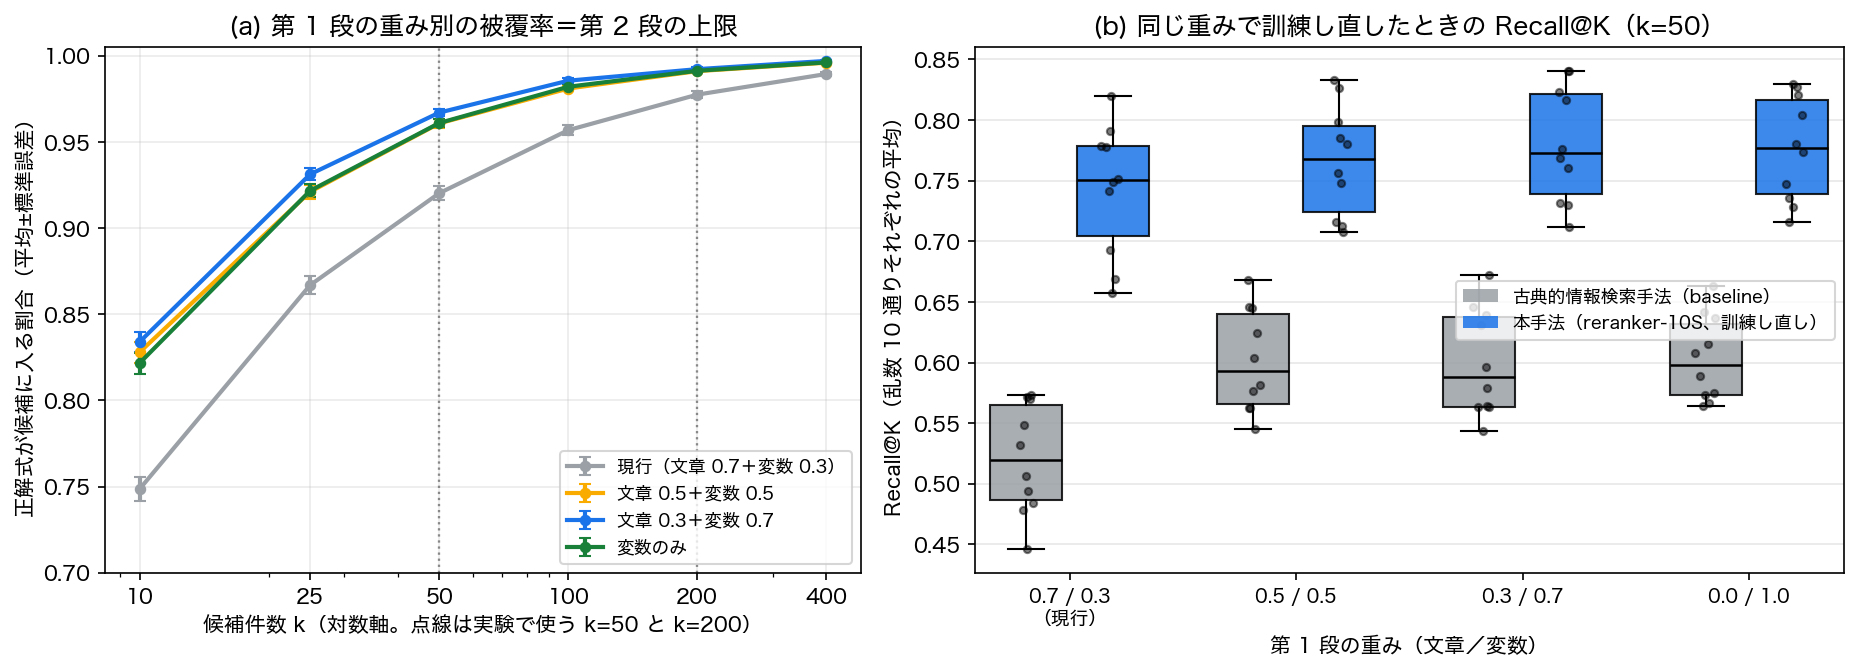
\includegraphics[width=0.98\linewidth]{figures/fig_stage1_redesign_ja.png}
\caption{第 1 段の重みを変える実験（設定 A）。(a) 重み別の被覆率（1{,}823 ケースの平均$\pm$標準誤差。点線は実験で使う $k=50$ と $k=200$）。(b) 候補作り・訓練・評価を同じ重みで行なったときの $\rk$（$k=50$。箱＝乱数 10 通りの四分位、横線＝中央値、点＝各乱数の値）。被覆率の順序と最終精度の順序が一致し、文章 $0.3$＋変数 $0.7$ が両方で最良になる。}
\label{fig:redesign}
\end{figure}

%======================================================================
\section{現時点の限界}\label{sec:limits}
%======================================================================
\begin{itemize}[leftmargin=1.5em]
  \item 合成ケースの説明文は LLM が書いたもので、人が書く依頼文と文体が違う可能性がある（式・入出力は規則で決まる）。
  \item 評価はデータベースの中に閉じており、データベースに無い式は検索できない。LLM 直接生成との比較は各設定約 50 件で、等価判定（別モデルによる機械判定）の人手検証は行なっていない。
  \item 変数の重なりを測る 6 特徴量だけで課題の大半が解ける（シャッフルで $0.68$ 低下）。これはケースを「変数を共有する式」から作った本データの性質も反映しており、表記の揺れた実文献のクエリへそのまま移るかは未検証である。
  \item 逐次の学習は正解を 1 本ずつ与える手順であり、推論時は自分の選択（誤り込み）を参照する。この食い違いは残っている。
\end{itemize}

%======================================================================
\section{まとめと今後の課題}
%======================================================================
\textbf{まとめ}：数式集合の検索は、候補を絞って（第 1 段）、集合として並べ直す（第 2 段）2 段構えで、$\rk$ を $0.521 \to 0.743$ に上げられる。効いている信号は変数の重なり（中でも式の特化度）であり、話題の近さはどの形でも効かない。その原因を「絞り込み後の冗長性・選抜の逆相関・打ち消し合い」として特定した。逐次選択は最難ケースの頭打ちを解き（$+0.056$）、自由度ゼロ停止は式の本数を教えられなくても解ける集合を返して止まる。誤りの過半が第 1 段で生まれると特定できたので、第 1 段を変数寄りに作り直したところ、予測どおり上限が上がり、$\rk$ は $0.780$（最強構成では $0.810$）まで伸びた。

\textbf{今後の課題}：
\begin{itemize}[leftmargin=1.5em]
  \item 残る誤りの 2 つの型のうち「式の向き」（どの変数を決める式か）を表す特徴量を設計する。
  \item 比較手法を増やす（BM25 などの標準的な検索手法、埋め込みベクトル検索）。
  \item LLM による等価判定の妥当性を、一部を人手で判定して確かめる。
\end{itemize}

\end{document}
